\documentclass[12pt]{article}
\usepackage[left=1in, right=1in, top=1in,bottom = 1in]{geometry}
\usepackage{amsmath}
\usepackage{xcolor}
\usepackage{lmodern}
\usepackage{listings}
\usepackage{graphicx}
\usepackage{float}

\lstset{language=[90]Fortran,
  basicstyle=\ttfamily,
  keywordstyle=\color{red},
  commentstyle=\color{blue},
  morecomment=[l]{!\ }% Comment only with space after !
}

\begin{document}
	\begin{flushleft}
		Max Le \\
		ID: 901223283\\
		MTH 5050: Parallel Process\\
		Assignment 2: Using MPI with Blueshark  
	\end{flushleft}


	\section{Problem Statement}
	
	The goal of this assignment is to modify the original code, where we try to numerically integrate $\displaystyle\dfrac{4}{1+x^2}$ from 0 to 1. This original code was given on Canvas. \newline\\
	The original code has 2 main steps that involve MPI: first, we use MPI BROADCAST to send the problem size from process 0 to the other processes; next,MPI REDUCE is used in order to collect the partial sum from all of the other processes back to process 0 and then sum them up to get our result. \newline\\
	We need to replace the BROADCAST and REDUCE functions by a series of SEND/RECV function. Then, we are going to perform speed up test and scaled efficiency test on both the original code and the modified code. 
	
	\section{Approach}
	
	From assignment 1, we know that our result should be close to $\pi \approx 3.1416...$.  Firstly, in order to replace BROADCAST with SEND/RECV, this is the pseudo code of how I am going to do it:
	
	\begin{itemize}
		\item  If process is 0, then send "n", the problem size, to other processes. This is done in a loop because we need process 0 to send "n" to do the SEND function multiple times. 
		\item  If process is not 0, then we just need one RECV call.  It will receive "n" from process 0. 
	\end{itemize}

	\noindent
	In code, this looks something like this: 
	\begin{lstlisting}
	if (rank == 0 ) then
	  ! SENDING FROM 0 to OTHERS
	  do i = rank+1,nproc-1
		call MPI_SEND(n,1,MPI_INT,i,1,&
			MPI_COMM_WORLD,ierr)
	  end do
	else
	    ! OTHERS RECEIVE 
		call MPI_RECV(n,1,MPI_INT,0,1,&
			MPI_COMM_WORLD,status1,ierr)
	end if		
	\end{lstlisting}
	\noindent
	The "1" after the "i" in the SEND call and after "0" in the RECV call is for the tag. This tag means that we are going to perform communications "1" where 0 send "n", and other processes receive "n" from 0. In contrast, in order to replace REDUCE with SEND/RECV, we have to do the opposite.  In pseudocode, it looks something like this: 

	\begin{itemize}
		\item If process is 0, we are going to receive the partial sum: "mypi" in this case. Then we are going to sum up. 
		\item Else, we are all going to send "mypi" to process 0 
	\end{itemize}
	\noindent
	In code, this looks something like this: 

	\begin{lstlisting}
	if (rank == 0) then 
	 ! RECEIVE mypi
	 do i = 1,nprocs -1  
	   call MPI_RECV(mypi_recv,1,MPI_DOUBLE_PRECISION,i,&
			2,MPI_COMM_WORLD,status1,ierr)
	   pi = pi + mypi    ! SUMMING UP
	 end do

	else
	  ! SEND mypi
	   call MPI_SEND(mypi,1,MPI_DOUBLE_PRECISION,0,&
			   2,MPI_COMM_WORLD,ierr)
	end if 
	\end{lstlisting}

	\noindent
	The tag is now "2".  This is to indicate that the communication is to send "mypi", not "n" from before. We are sending/receiving "mypi".  It is also important to note that if we want to use "pi" as the final storage, then we need an extra step before this.  Basically, if process is 0, then "pi" is "mypi" and then if we happen to fall into the above algorithm (have more than 1 process), then "pi" would get updated.  

	\begin{lstlisting}
	if (rank == 0) then 
		pi = mypi  ! STORE mypi into pi at process 0
	end if     
	\end{lstlisting}
	\noindent
	The time is calculated with MPI WTIME, the clock starts when we set problem size for process 0, and end when we finish.  In order to get better timing, the code is executed 5 times for each case and for each processor.  Then the average time is used to compute speed up/ scale efficiency. \\
	\noindent
	The speed up is calculated as:  $ \dfrac{\textrm{Time takes to run fixed N for 1 process}}{\textrm{Time takes to  run fixed N for multiple processes}}$
	\newline
	\newline
	\newline
	\noindent
	Meanwhile, the scale efficiency = $\dfrac{\textrm{Time to run for 1 process at N0 problem size}}{\textrm{Time to run for P processes at NP problem size}}$.\\ \\
	\noindent
	where the ratio of interval per process is kept to be 100,000,000. 

	\newpage
	\section{Results}
	\subsection{FIXED N}
	\subsubsection{Time results for fixed N = 800,000,000 for different number of processors}

	\begin{center}	
	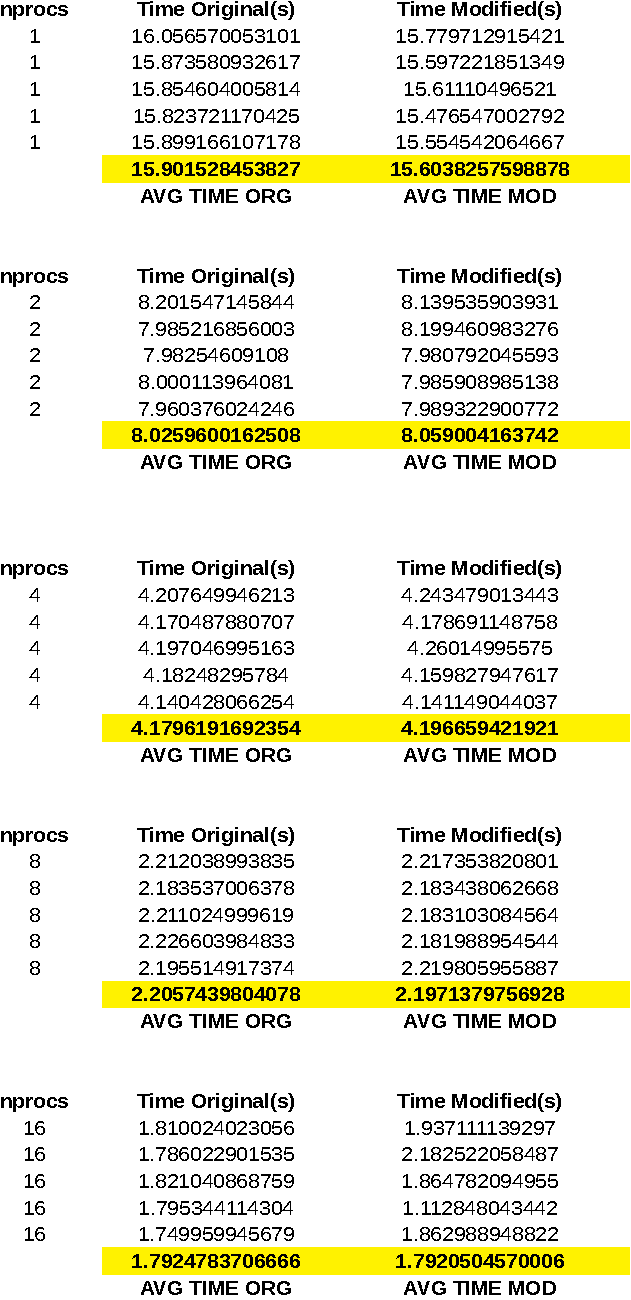
\includegraphics[width = 120mm,height = 200mm]{fixedN_alltime-crop}
	\end{center}

	\newpage
	\subsubsection{Average time, errors, numerical values, and speed up calculation for fixed N}
	\begin{center}	
		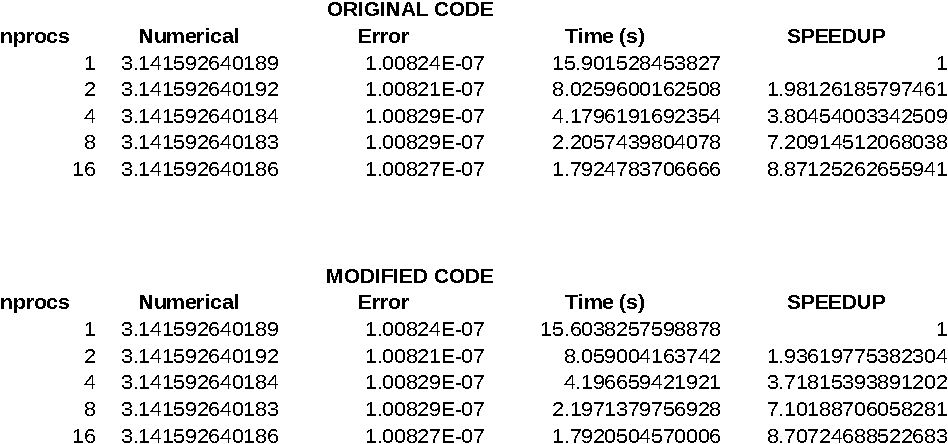
\includegraphics[width = 150mm,height = 80mm]{fixedN_final-crop}
	\end{center}
	
	\subsubsection{Plots comparing original and modified code fixed N}

	\begin{figure}[H]
		\hfill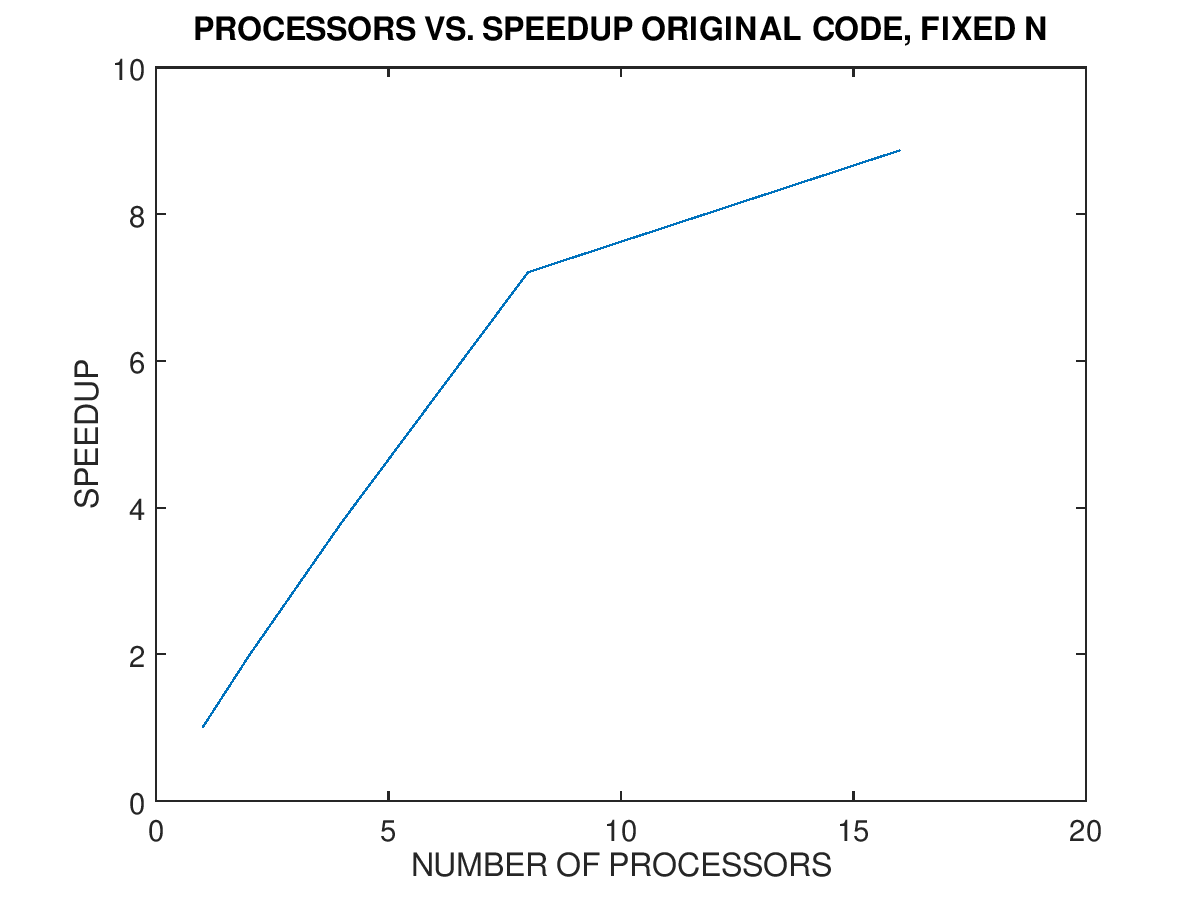
\includegraphics[width=150mm,height= 100mm]{fix_ori.png}\hspace*{\fill}
		\caption{Original code speed up fixed N}
	\end{figure}



	\begin{figure}[H]
		\hfill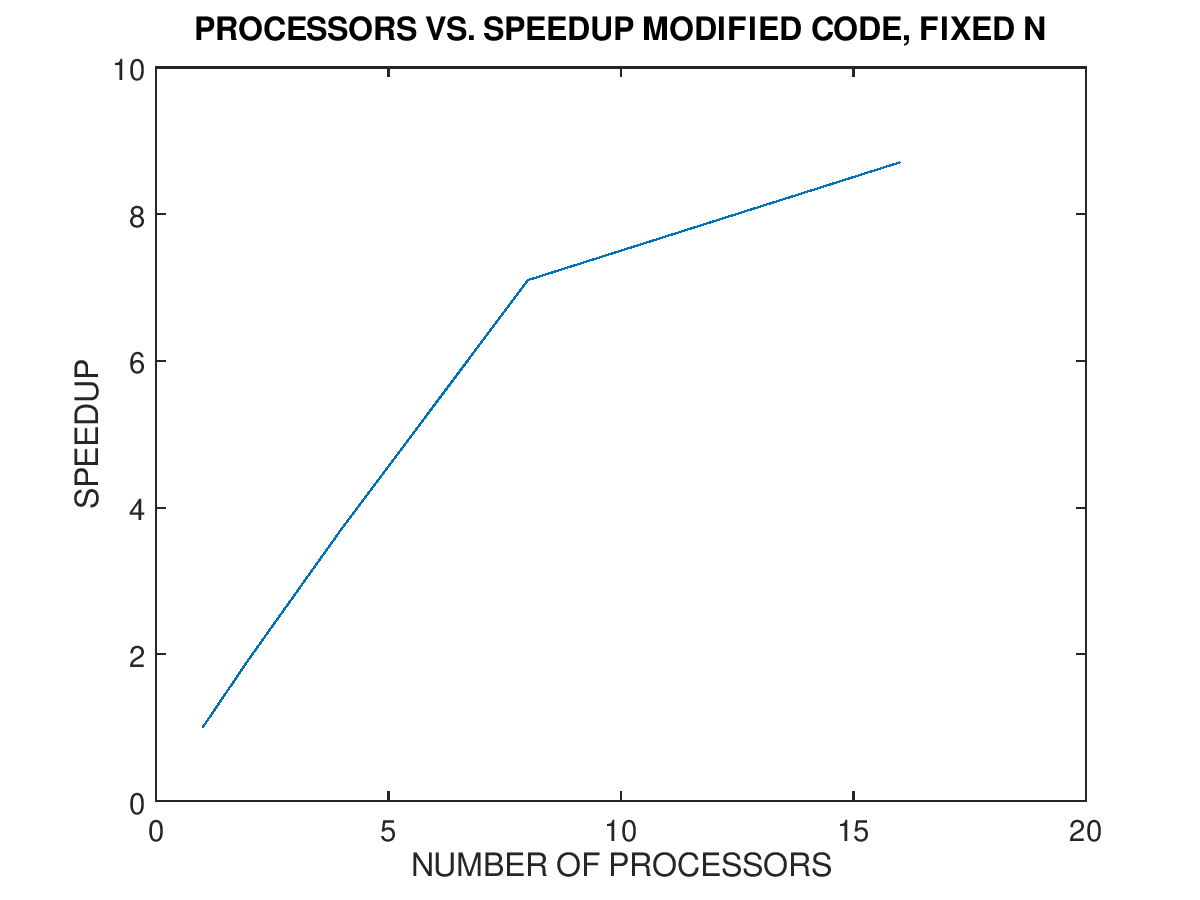
\includegraphics[width=150mm,height= 100mm]{fix_mod.png}\hspace*{\fill}
		\caption{Modified code speed up fixed N }
	\end{figure}


	\begin{figure}[H]
		\hfill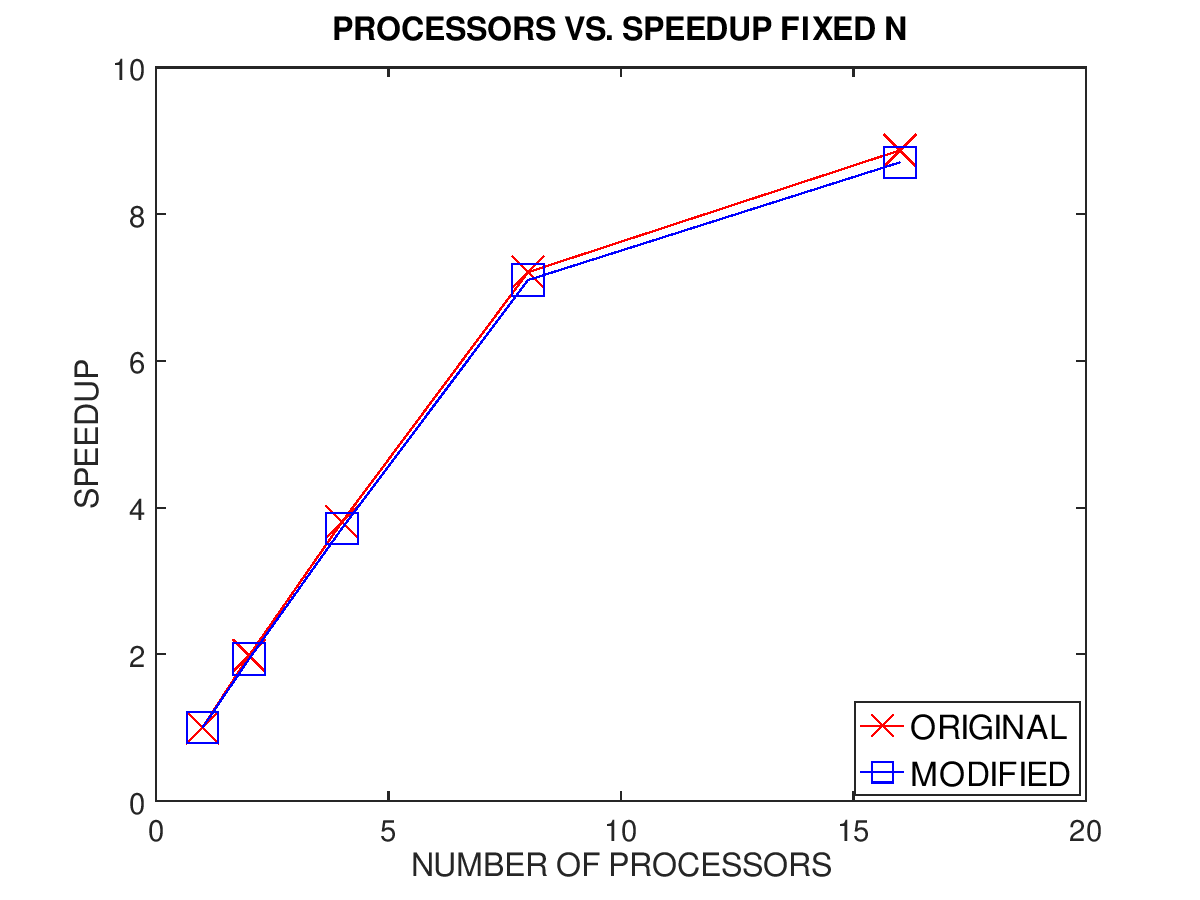
\includegraphics[width=150mm,height= 100mm]{fix_combine.png}\hspace*{\fill}
		\caption{Original vs. Modified speed up fixed N }
	\end{figure}

	\newpage
	\subsection{VARIED N}
	\noindent
	\subsubsection{Time results for varied N for different number of processors} 
	\begin{center}	
	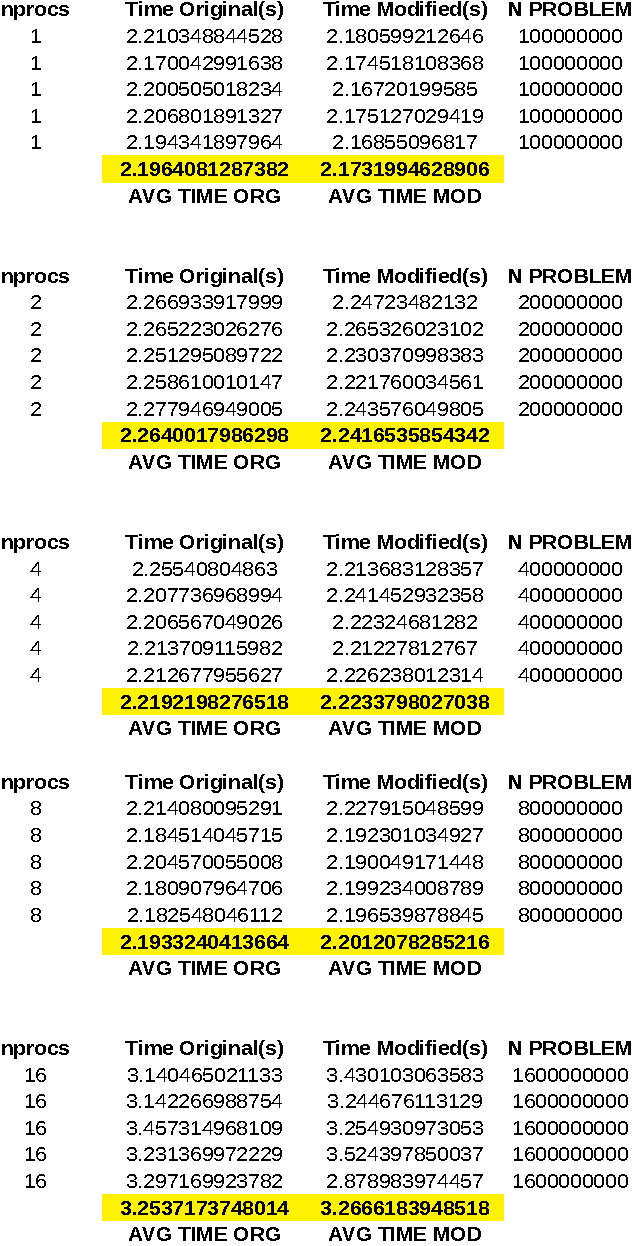
\includegraphics[width = 120mm,height = 200mm]{variedN_alltime-crop}
	\end{center}

	\subsubsection{Average time, errors, numerical values, and speed up calculation for varied N}

	\begin{center}	
		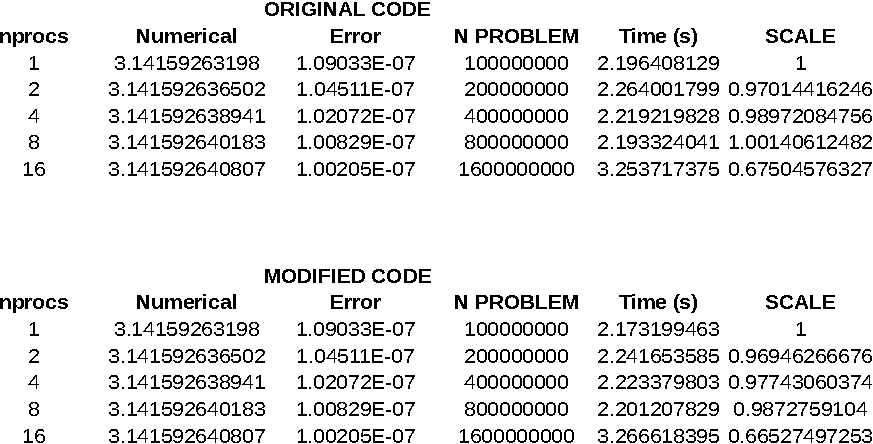
\includegraphics[width = 150mm,height = 80mm]{variedN_final-crop}
	\end{center}

	\subsubsection{Plots comparing original and modified code varied N}

	\begin{figure}[H]
		\hfill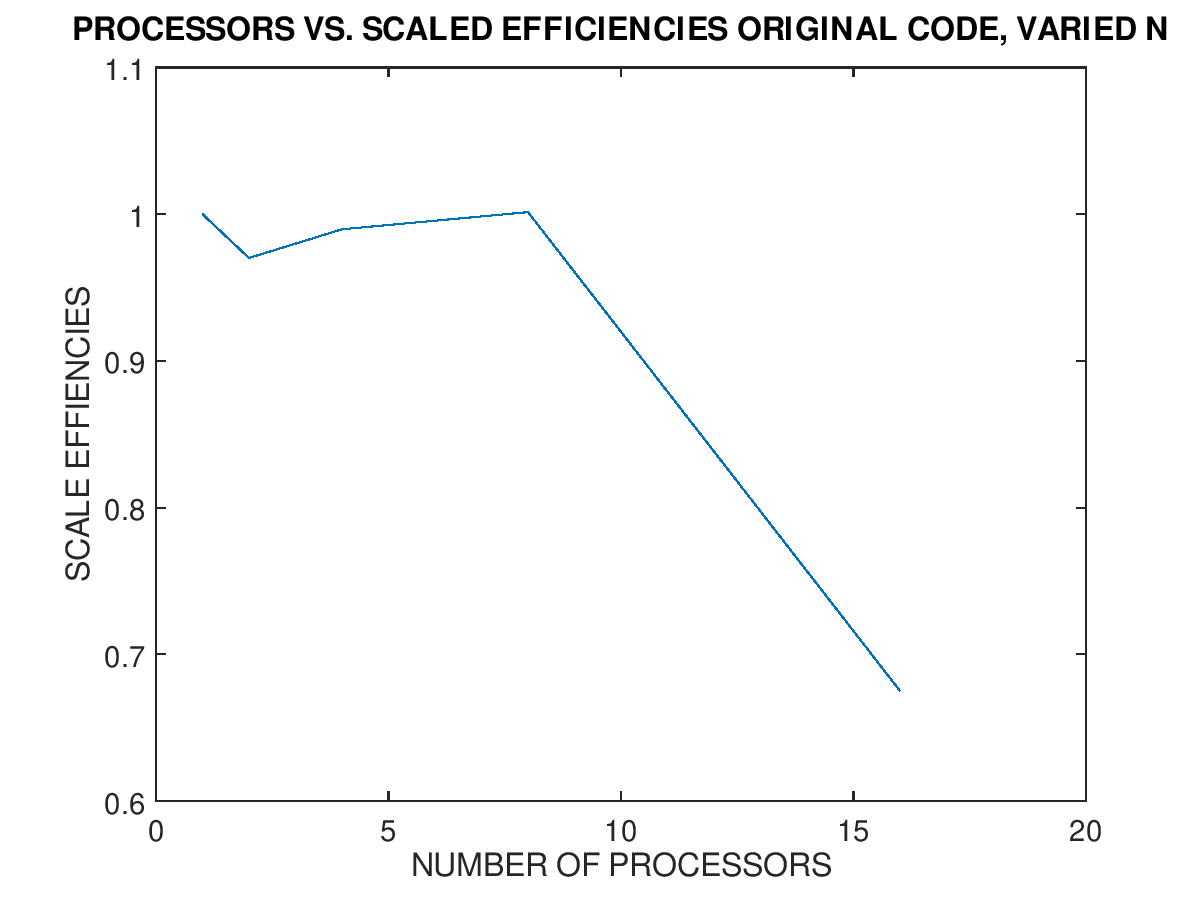
\includegraphics[width=150mm,height= 100mm]{varied_ori.png}\hspace*{\fill}
		\caption{Original code speed up varied N}
	\end{figure}

	\begin{figure}[H]
		\hfill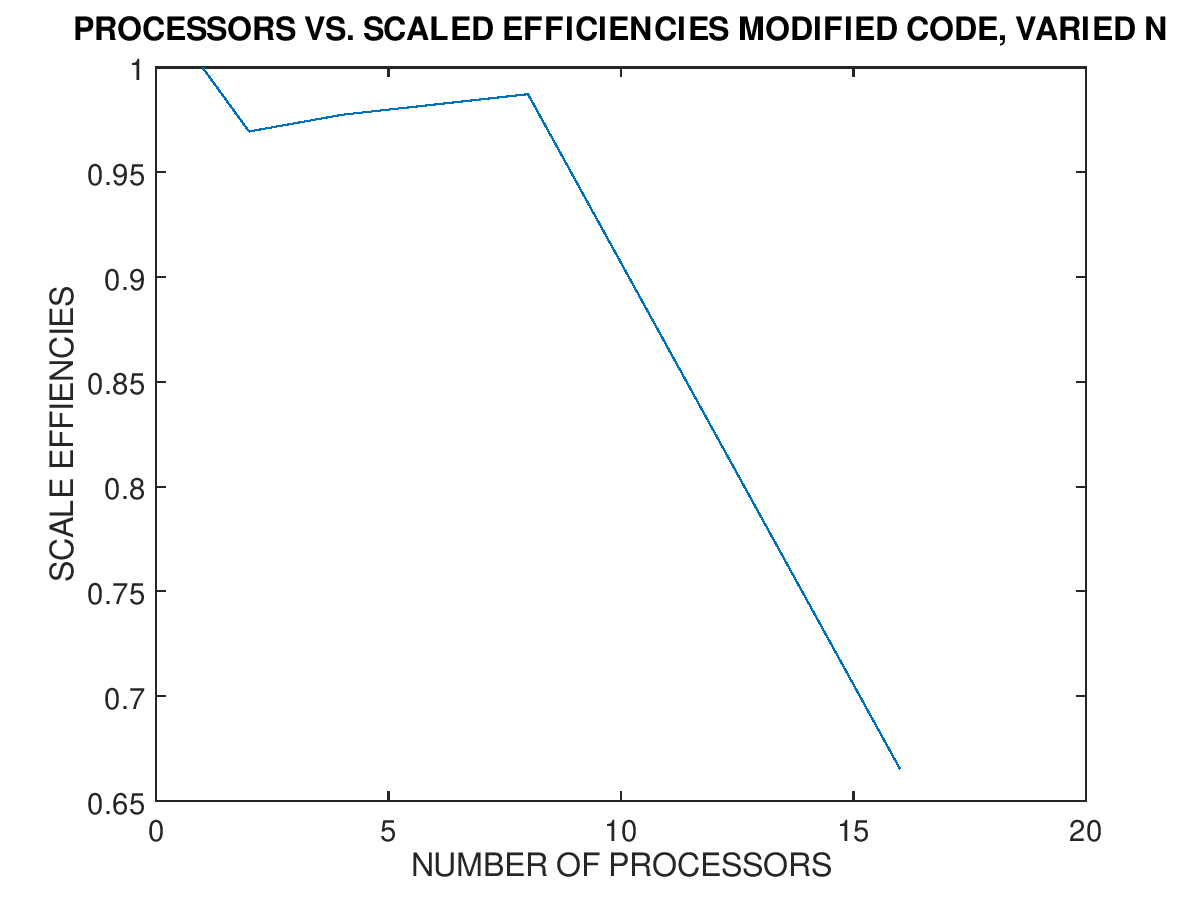
\includegraphics[width=150mm,height= 100mm]{varied_mod.png}\hspace*{\fill}
		\caption{Modified code speed up varied N }
	\end{figure}


	\begin{figure}[H]
		\hfill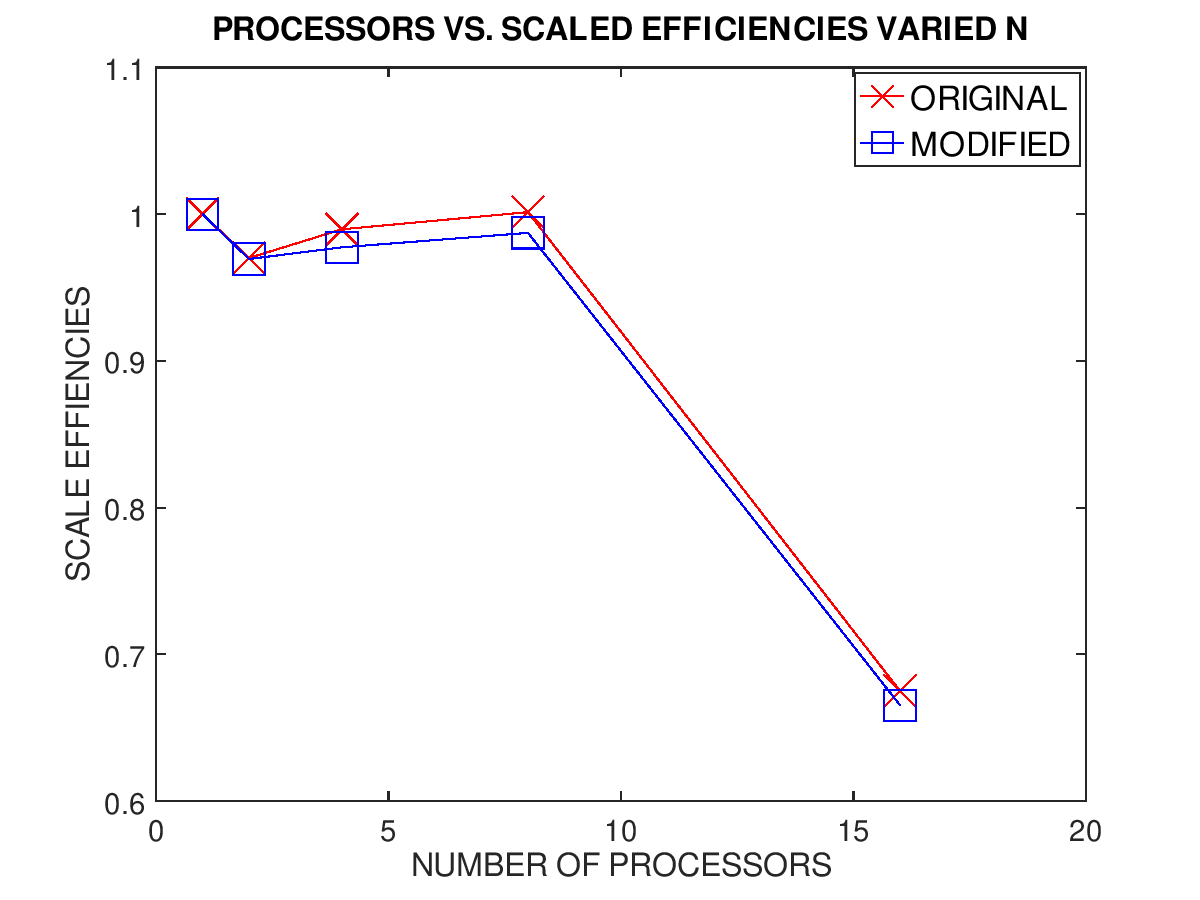
\includegraphics[width=150mm,height= 100mm]{varied_combine.png}\hspace*{\fill}
		\caption{Original vs. Modified speed up varied N }
	\end{figure}

	\section{Discussion}

	\subsection{Speed Up Study}
	For the speed up study, theoretically, perfect speed up is achieved when Speed Up = Number of Processors. We can see from Figure 1 to 3 that perfect speed up is almost achieved when using 2,4 and 8 processors. For example, for 8 processors, we got 7.1 as a speed up factor, this is close to 8, making it almost a perfect speed up.  The same thing can be said about 2 and 4 processors.  Unfortunately, 16 processors do not show the same trend. We are getting around 8.7 as speed up factor for 16 processors.  This is not very efficient because we can just get the same speed up factor as 8 instead, without spending more resources on using 16 processors. 

	\subsection{Scaled Efficiency}
	In contrast to the speed up test, perfect scaling is achieved when Scaling = 1.  This means that our work rate to solve a similar problem is the same.  In other words, because the number of intervals per process is kept constant; we should expect the time it takes to solve the problem to be similar. This is true if we look at Figure 4,5 and 6. For 2, 4, and 8 processors, the scaled efficiencies flunctuate around 1. Now, this is clearly not the case for 16 processors, the scaled efficiency is only 0.67 for both original code and modified code. It looks as if our work rate to solve the problem gets diminished. One possible explanation for this outlier in both Speed Up and Scaled Efficiency has to do with hardware problems. The Blueshark cluster has 2  times Hexa-Core Intel Xeon X5650, this means 12 cores per node. Therefore, if we are requesting more than 12 processors, in this case 16, then the cluster might not request the correct number of processors. Thus, for the Speed Up test, we don't have enough power (processors) to solve. On the other hand, for the Scaled Efficiency test, our code requests a large problem size; however, because of the hardware, we do not have enough resources to solve such large problem. 

	\subsection{Modified vs Original}

	In both test cases, the original is better.  For example, using 8 processors, the original code has a closer value of speed up factor to being "perfect", 8, than the modified code.  The same thing can be said about the scaled efficiency test, the original code has closer efficiency value to 1.0 than the modified one. One possible explanation would be that the Broadcast and Reduce functions are well written for numerical integrations, i.e sending problem size and then collect them all back.  The send/receive functions can replace the original bcast/reduce; however, it is not very efficient.  One way to think about this is that to we need a Do/For loop for sending problem size "N" from process 0 to all of the other processors. It could be that the Do/For loop in Bcast/Reduce is written better and therfore is optimized. Although, the difference is not that great: original code is only slightly better than the modified one. If optimization is true for Bcast/Reduce, then we should see a more drastic difference between the original and modified code when we solve large problems where there are needs to send and receive large amount of data between processors. 

	\section{Code}


	\begin{lstlisting}

program midpoint_speedup
   
    	include 'mpif.h'
   
	integer :: ierr, rank, nprocs,n,i, isend, nsend, nreceive
	integer,dimension(MPI_STATUS_SIZE) :: status1
	double precision :: real_PI
	double precision :: mypi, pi, h, sum, x
	double precision startwtime, endwtime
	double precision :: mypi0, mypi_recv

	startwtime = 0.0
	real_PI = 3.141592653589793238462643

	!Start OPENMP
	call MPI_INIT(ierr)
	call MPI_COMM_SIZE(MPI_COMM_WORLD,nprocs,ierr)
	call MPI_COMM_RANK(MPI_COMM_WORLD,rank,ierr)


	n = 0
	! SET PROBLEM SIZE AT PROCESS 0
	if (rank == 0) then
		! Change this for varied N, or fixed N
		!n =  800000000
		n = nprocs*100000000
		startwtime =  MPI_WTIME()
	end if

    !************** SEND/RECEIVE PROBLEM SIZE FROM 0  ********** !
    ! SEND CALL
    if (rank == 0) then
        do i = 1,nprocs-1
            call MPI_SEND(n,1,MPI_INT,i,1,MPI_COMM_WORLD,ierr)
        end do
    ! RECEIVE CALL
    else
        call MPI_RECV(n,1,MPI_INT,0,1,MPI_COMM_WORLD,status1,ierr)
    end if


    !***************** MID POINT CODE ************************! 
    ! COMPUTE PARTIAL SUM
    h = 1.0/(1.0*n)
    sum = 0.0
    do i = rank+1,n,nprocs
        x = h*((1.0)*i-0.5)
        sum = sum + 4.0/(1.0+x*x)
    end do
    mypi = h*sum
    if (rank == 0) then 
        pi = mypi
    end if
    
    !*************** SEND MY PI TO ZERO TO SUM UP  ****************!        
    if (rank == 0) then
        do i = 1,nprocs-1
            ! receive my pi
	    call MPI_RECV(mypi_recv,1,MPI_DOUBLE_PRECISION,i,2,&
				MPI_COMM_WORLD,status1,ierr)
            pi = pi + mypi_recv
        end do
    else
        ! send mypi
	call MPI_SEND(mypi,1,MPI_DOUBLE_PRECISION,0,2,&
				MPI_COMM_WORLD,ierr)
    end if


    !**********  WRITE RESULT *******************************!
    if (rank == 0) then
        endwtime =  MPI_WTIME()
        write (6,200) pi, abs(pi-real_PI), nprocs
	200 format(' ','pi is approximately ',f16.12,',Error is ',&
			f16.12,' nprocs = ', I2)
        write (6,300) endwtime-startwtime
    300 format(' ','wall click time = ', f16.12)
	write(6,400) n
    400 format(' ','N SIZE = ', I10) 

    end if

    ! Close OPENMP
    call MPI_FINALIZE(ierr)
end program midpoint_speedup





		
	\end{lstlisting}

	

	
\end{document}